\documentclass[11pt,a4paper]{article}
\usepackage[margin=2cm]{geometry}
\usepackage{graphicx,booktabs,float,caption,parskip}
\usepackage[T1]{fontenc}
\usepackage{lmodern}
\usepackage[hidelinks]{hyperref}
\usepackage[htt]{hyphenat}
\captionsetup{font=small,labelformat=empty}
\newcommand{\psid}[1]{\includegraphics[width=\linewidth,height=0.62\textheight,keepaspectratio]{figures/main/#1}}
\newcommand{\ukhls}[1]{\includegraphics[width=\linewidth,height=0.80\textheight,keepaspectratio]{../../paper/figures/#1}}
\newcommand{\fig}[2]{\clearpage\section*{Figure #1: #2}}
\newcommand{\orig}[1]{\clearpage\subsection*{UKHLS original, for comparison}\begin{center}\ukhls{#1}\end{center}}

\begin{document}
\begin{center}
{\Large\bfseries The paper's main-text figures on PSID data}\\[4pt]
PSID 2003 to 2023, biennial waves; no Bayesian models\\[2pt]
\small Built by the scripts in \texttt{descriptives/psid/}, 5 November 2026
\end{center}

Each main-text figure of \texttt{paper/paper\_skeleton.tex} (Figures 1 to 15), and appendix Figure B.1 (the measure), which comes first, is listed below as replicated (the same exercise on PSID), adapted (the Bayesian content replaced by partial K-means, the paper's non-parametric types) or skipped. For each figure that is drawn there follows the PSID version with a caption, a note on what differs from the UKHLS version and what the comparison shows, and then the UKHLS original from \texttt{paper/figures/}.

\begin{center}\footnotesize
\begin{tabular}{r p{4.6cm} p{3.6cm} p{6.2cm}}
\toprule
& Figure & Status & PSID script \\
\midrule
B.1 & the measure: $h$ against $\theta$, item thresholds & replicated & \texttt{21\_psid\_health\_scale.py} \\
1 & cost and mortality against $\theta$ & replicated & \texttt{37\_psid\_cost\_mortality\_age.py} \\
2 & Exhibit 1: moments over the lifecycle & replicated & \texttt{23\_psid\_exhibit1.py} \\
3 & Exhibit 2: Case 4 moments & replicated & \texttt{29\_psid\_moments.py} \\
4 & partial K-means types, $K=3$ & replicated & \texttt{22\_psid\_kmeans.py}, \texttt{25\_psid\_clusters.py} \\
5 & between versus within by age & replicated & \texttt{25\_psid\_clusters.py} \\
6 & $K=3$ Bayesian mixtures & skipped & Bayesian; its K-means content is Figure 4 \\
7 & class trajectories by $K$ & adapted: K-means at $K=3,4,5$ & \texttt{36\_psid\_trajectories\_kmeans.py} \\
8 & multidimensional mixture, cohort shifts & skipped & Bayesian and multidimensional \\
9 & multidimensional against univariate & skipped & Bayesian and multidimensional \\
10 & types over age windows & adapted: K-means windows & \texttt{26\_psid\_windows.py} \\
11 & predicting death & adapted: $\theta$ and K-means only & \texttt{33\_psid\_prediction.py}, \texttt{41\_psid\_mortality\_prediction.py} \\
12 & trajectories by type and observables & adapted: K-means in (a) & \texttt{27\_psid\_observables.py} \\
13 & predicting ahead and the type & adapted: $\theta$, observables, K-means & \texttt{33\_psid\_prediction.py}, \texttt{43\_psid\_type\_from\_initial.py}, \texttt{56\_psid\_prediction\_summary.py} \\
14 & prevention & adapted: K-means types & \texttt{47\_psid\_prevention.py} \\
15 & prevention and life expectancy & skipped & multidimensional Bayesian fit, Gompertz--Makeham, ONS tables \\
\bottomrule
\end{tabular}
\end{center}

\subsection*{What is common to every PSID figure}
\begin{itemize}\itemsep2pt
\item \textbf{Measure.} $\theta$ is the five-testlet graded-response measure asked in every PSID wave (\texttt{data\_cleaning/psid/02\_build\_psid\_health.py}), pooled $N(0,1)$ on PSID. It is not the UKHLS $\theta$: the items differ, and each is standardised on its own sample, so levels and units are comparable in shape, not in value.
\item \textbf{Sample.} The PSID contract mirrors the UKHLS one: Reference Persons and Spouses, ages 20 to 89, one row per person-age, people with at least three observed ages: 18,486 people (38,963 in the UKHLS). Because waves are two years apart, three observations span at least four years.
\item \textbf{Timing.} A PSID ``wave ahead'' is two years, death before the next wave is death within two years, and within-person lags are mostly even. Where the paper uses one-year steps, the PSID figures use the lags PSID has and say so.
\item \textbf{Cost.} PSID has no GP or out-patient counts. The PSID index prices non-maternity hospital nights in the calendar year before the interview at the UKHLS index's stage 1 NHS rates (0 to 1 nights at the non-elective short-stay price, \pounds826; longer stays at \pounds791 per bed day), one admission per year with any nights. It is an in-patient index; the UKHLS index adds out-patient and GP contacts.
\item \textbf{Observables.} Education is \texttt{educ\_best} in four US groups (less than high school, high school, some college, bachelor's or more); income is the mean within-wave rank of equivalised family income; region is the four census regions; ethnic group is white, Black, Hispanic, Asian, other.
\item \textbf{Partial K-means} uses the repo's own \texttt{partial\_kmeans} with the paper's settings (50 seeded starts, types ordered worst to best). The K-means runs take about 40 seconds in parallel; every other script runs in under five seconds.
\end{itemize}

%-----------------------------------------------------------------
\fig{B.1}{The measure (appendix)}
\begin{center}\psid{fig_health_scale.png}\end{center}
\textbf{Caption (PSID).} The measure. (a) The expected-score curve mapping $\theta$ to $h$, over the pooled distribution of $\theta$; (b) each testlet's discrimination against its thresholds. 144,687 person-waves, 2003 to 2023.

\textbf{What differs.} PSID has five testlets asked in every wave, against eight in the UKHLS: general health (GH, five categories), role limitation (RP), the two functional-limitation testlets (LIM\_FL, LIM\_SELF, both binary in PSID) and the condition count (COND, eight categories). There is no physical-functioning (PF), bodily-pain (BP) or sensory (LIM\_SENS) testlet; PSID asks a PF-like mobility item only from 2017, used in the six-testlet check measure, not here. The score is therefore much coarser: 580 distinct values of $\theta$ against 28,360 in the UKHLS, and 11.5 percent of person-waves at the ceiling against 7.2 percent (UKHLS figures from \texttt{artifacts/descriptives/health\_measure\_properties.csv} and \texttt{ceiling\_floor.csv}).

\textbf{What the comparison shows.} Both measures pile up at a ceiling, the PSID one at $\theta \approx 1.3$ ($h \approx 0.95$) and the UKHLS one near 0.9, and the PSID ceiling holds more people. With fewer and coarser items the PSID distribution is lumpier, and its $h$ curve is less of a clean logistic: it rises steeply up to $\theta \approx -1$ and then flattens, since above that only GH and the upper COND thresholds still discriminate. The two limitation testlets discriminate most ($a$ of 4.5 and 3.7, against at most 3.6 in the UKHLS) but each speaks at a single point, around $\theta = -1.4$ and $-1.9$; GH and COND cover the healthy half of the range, as in the UKHLS. The point to carry into the other figures: a unit of PSID $\theta$ is not a unit of UKHLS $\theta$, and the PSID scale says less about differences among the healthy.
\orig{fig_health_scale.png}

%-----------------------------------------------------------------
\fig{1}{Cost and mortality against $\theta$, by age band}
\begin{center}\psid{fig_cost_mortality_age.png}\end{center}
\textbf{Caption (PSID).} (a) Mean annual in-patient cost index in equal-width bins of $\theta$ within three age bands, with 95 percent intervals; the orange line is the pooled cubic in $\theta$ that the PSID prevention figure prices with; grey circles are the UKHLS in-patient tier in the same bins, all ages pooled. (b) The two-year death rate in the same bins on a log scale, with the within-band logit drawn through it; ages 20 to 44 are left out of (b).

\textbf{What differs.} In-patient cost only, and the stays refer to the previous calendar year; mortality is over two years (1,913 deaths in 131,711 person-waves at risk, waves 2003 to 2021), so rates are roughly double the UKHLS one-year rates.

\textbf{What the comparison shows.} The shape carries over: cost is convex in $\theta$ and the bins for the three age bands lie on one curve, so the cost of a given health state hardly changes with age (pooled curvature $t = 30.6$; its change per decade of age $t = 2.7$, against 33.5 and 3.6 in the UKHLS). Mortality is log-linear in $\theta$ with a gradient that flattens slightly with age ($t = -1.7$, against $-1.9$). The PSID in-patient cost at the sick end, around \pounds7,000 to \pounds8,000 a year at $\theta \approx -2.5$, is three to four times the UKHLS in-patient tier in the same bins. The two $\theta$ scales are not the same (each is standardised on its own sample and items), so the bins are not the same health states; longer stays or a different recall of nights in PSID may also contribute. I have not separated the two; the pooled cubic is $159 - 244\theta + 374\theta^2 - 203\theta^3$ pounds. Any-stay rate 8.0 percent; mean \pounds491 a year.
\orig{fig_cost_mortality_age.png}

%-----------------------------------------------------------------
\fig{2}{Exhibit 1: the measure's mean path, variance profile and covariance rows}
\begin{center}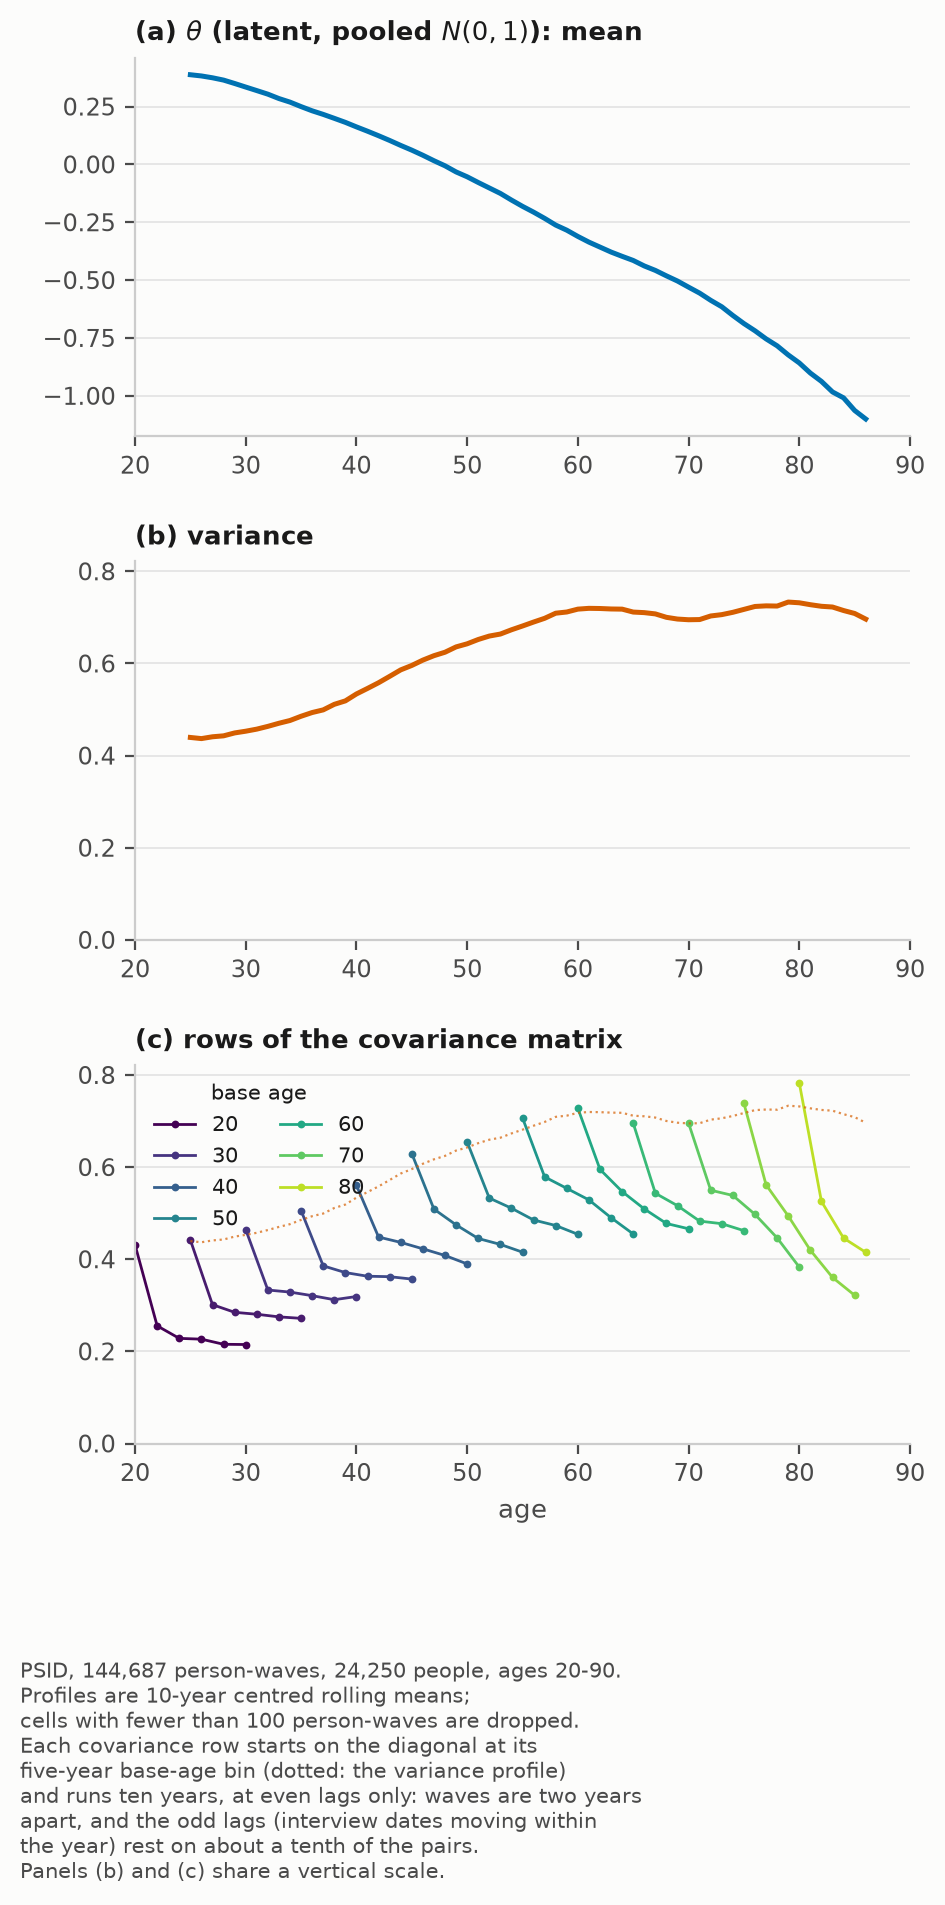
\includegraphics[height=0.62\textheight,keepaspectratio]{figures/main/fig_exhibit1.png}\end{center}
\textbf{Caption (PSID).} $\theta$'s mean path, variance profile and covariance rows, model-free. 144,687 person-waves; ten-year centred rolling means; each covariance row starts on the diagonal at a five-year base age and runs ten years, at the even lags.

\textbf{What differs.} Rows step in two-year lags. Odd lags exist (interview dates move within the year) but rest on about a tenth of the pairs and make the rows saw-toothed, so they are dropped from the figure and kept in the csv. Rows run ten years so the lag-8 and lag-10 points are kept.

\textbf{What the comparison shows.} The same three facts: a mean that falls steadily and faster after 70, a variance that rises from about 0.44 at 25 to 0.70 by 60 and is then flat, and rows that drop sharply off the diagonal (a large transitory component) then decline slowly, with the level of the rows rising with base age. The first off-diagonal drop is a two-year one here, so it mixes the one-period error with two years of decay of the persistent part.
\orig{fig_exhibit1.png}

%-----------------------------------------------------------------
\fig{3}{Exhibit 2: the linear approximation, Case 4}
\begin{center}\psid{fig_exhibit2_main.png}\end{center}
\textbf{Caption (PSID).} The ten moments of four ages four years apart in each band, pairwise moments, decomposed into the fitted layers under Case 4; properly constrained fit. 16,308 people with at least four observed ages.

\textbf{What differs.} Nothing in the design: four years apart sits on every second PSID wave. The ``one-period error'' is a two-year one, and the samples are a third to a sixth of the UKHLS ones (1,954 people in the 75 to 90 band).

\textbf{What the comparison shows.} $\rho$ is between 0.89 and 0.94 in every band (0.85 to 0.94 in the UKHLS). Corr$(H,d)$ is positive at 25 to 40 (0.17; 0.45 in the UKHLS) and negative at 60 to 75 ($-0.28$; $-0.56$), the same sign pattern of divergence then convergence. At 40 to 60 and 75 to 90 the constraint binds in PSID ($+1$ and $-1$), so only the sign is identified there; the UKHLS bands are interior ($+0.78$, $-0.53$). The signs agree in all four bands.
\orig{fig_exhibit2_main.png}

%-----------------------------------------------------------------
\fig{4}{Partial K-means types ($K=3$) on $\theta$}
\begin{center}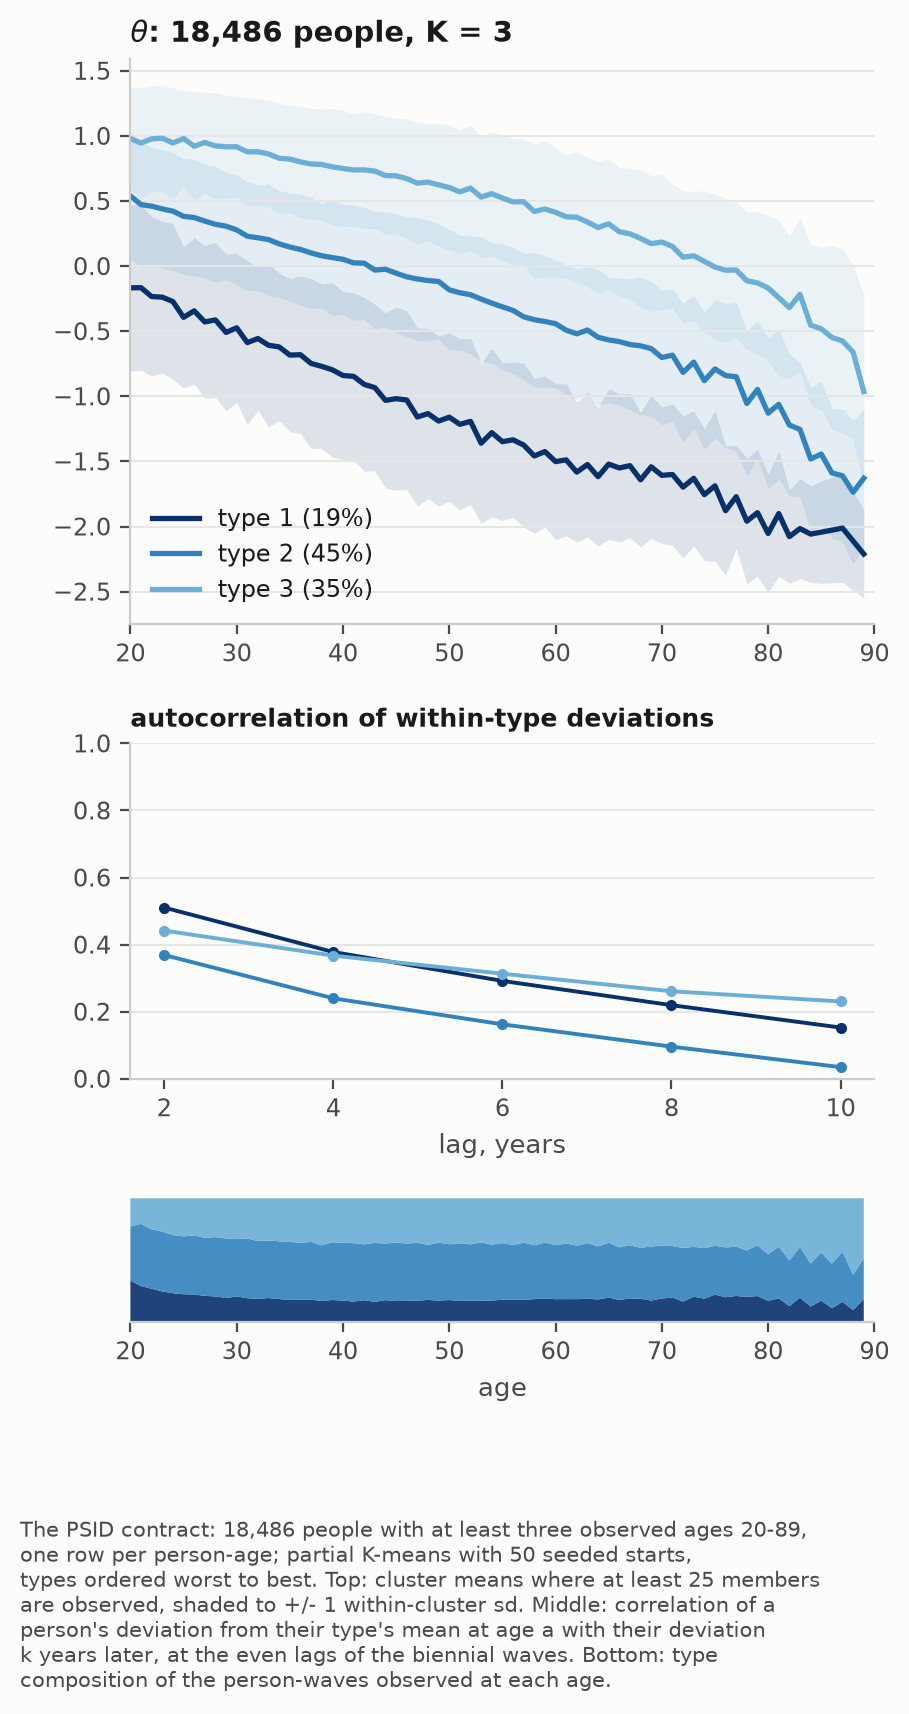
\includegraphics[height=0.62\textheight,keepaspectratio]{figures/main/fig_clusters.png}\end{center}
\textbf{Caption (PSID).} Top: type means with the within-type $\pm1$ sd band; middle: autocorrelation of within-type deviations by lag (even lags); bottom: type composition of the person-waves observed at each age.

\textbf{What differs.} The autocorrelation is at lags 2 to 10 years, not 1 to 9.

\textbf{What the comparison shows.} The typology is close to the UKHLS one. Shares are 19.5, 45.3 and 35.2 percent (18.0, 42.5, 39.5 in the UKHLS). Type means at 50 are $-1.16$, $-0.18$ and $0.60$. The worst type keeps the most persistent deviations (autocorrelation 0.51 at two years, 0.38 at four; UKHLS 0.56 and 0.44 at the same lags), the middle type the least.
\orig{fig_clusters.png}

%-----------------------------------------------------------------
\fig{5}{Between versus within by age, K-means types}
\begin{center}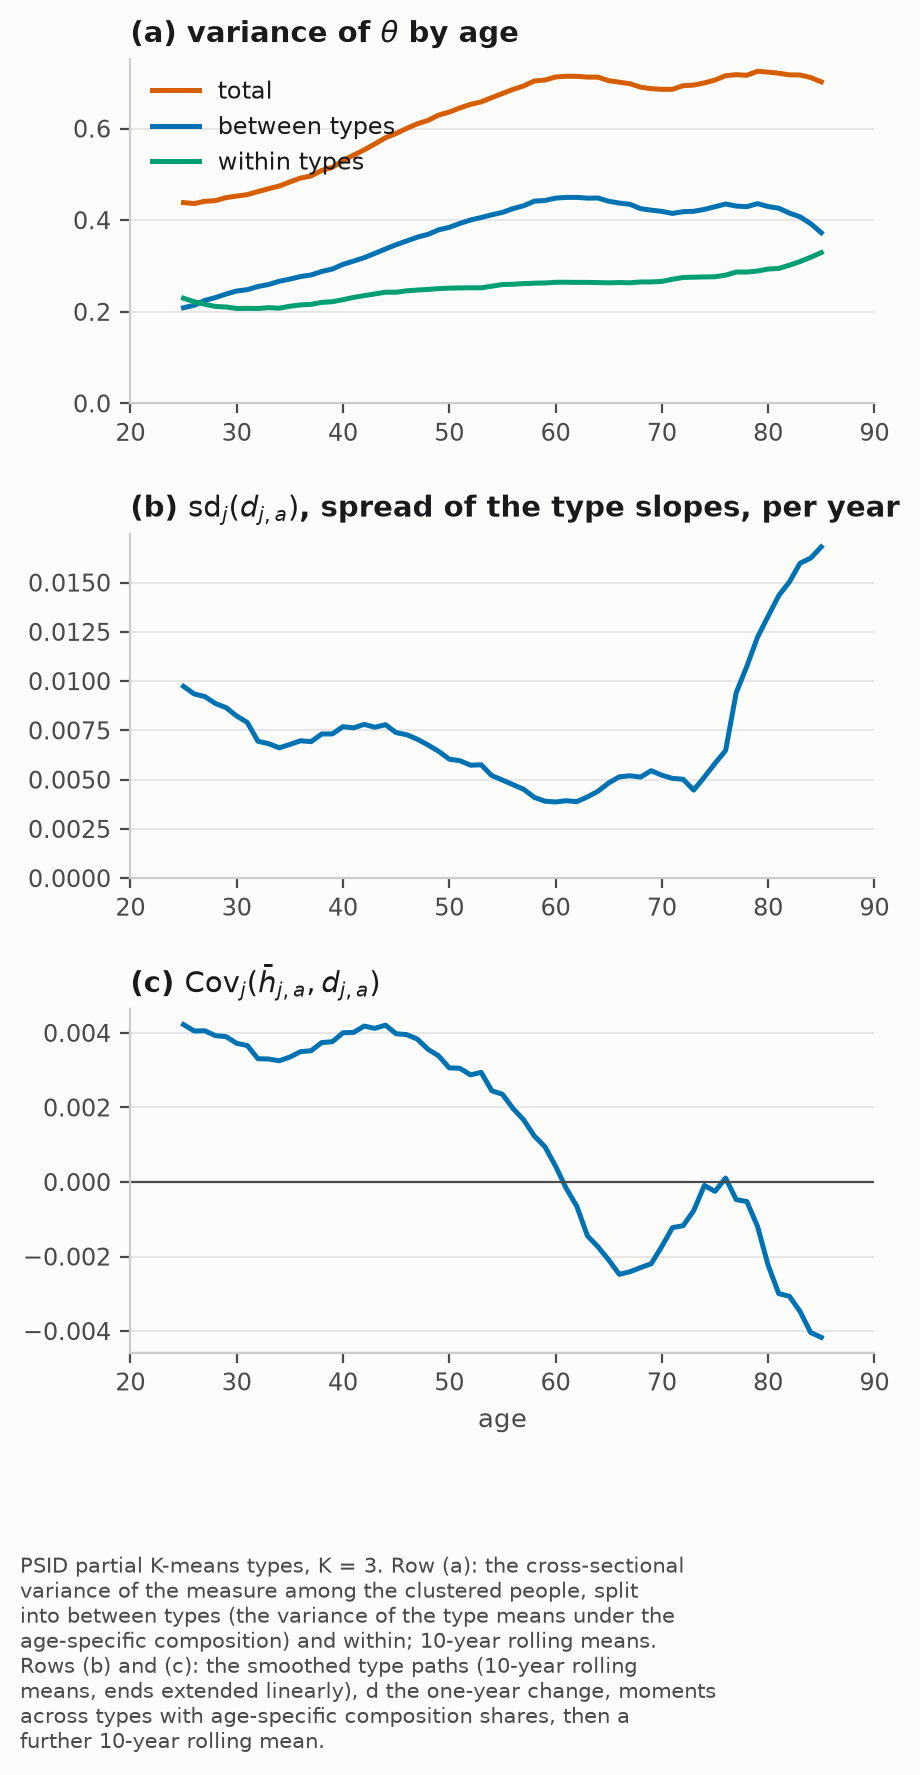
\includegraphics[height=0.62\textheight,keepaspectratio]{figures/main/fig_cluster_decomposition.png}\end{center}
\textbf{Caption (PSID).} (a) The cross-sectional variance split into between types and within; (b) the spread of the type slopes, sd$_j(d_{j,a})$, per year; (c) the level-slope covariance across types. Ten-year rolling means; age-specific composition shares.

\textbf{What differs.} Nothing beyond the data; slopes are one-year changes of the smoothed type paths as in the paper.

\textbf{What the comparison shows.} The types carry the same share of the variance: between-type share 0.55 at 30, 0.60 at 50, 0.61 at 70 (UKHLS 0.48, 0.59, 0.65). PSID has lower total variance at every age (0.64 at 50 against 0.76). The level-slope covariance turns from positive to negative around 60 in both, so the types diverge until about 60 and converge after. The rise in the PSID slope spread past 75 comes from the ends of the smoothed type paths, where few members of each type remain, and should not be read.
\orig{fig_cluster_decomposition.png}

%-----------------------------------------------------------------
\clearpage\section*{Figure 6: $K=3$ mixtures on $\theta$}
\textbf{Skipped.} The figure is two Bayesian growth mixtures (independent residuals and AR(1) plus ``spike''); no Bayesian model is fitted on PSID. Its K-means content, the type means on the same rows, is Figure 4.

%-----------------------------------------------------------------
\fig{7}{Type trajectories and shares by number of types (adapted)}
\begin{center}\psid{fig_class_trajectories_by_K.png}\end{center}
\textbf{Caption (PSID).} Partial K-means types on $\theta$ at $K=3$, 4 and 5. Line width is proportional to the type share, given in the legend; the strip beneath each panel is the type composition of the person-waves observed at each age. One vertical scale.

\textbf{What differs.} The paper draws Bayesian growth mixtures (two rows, two stochastic specifications); this is the K-means stand-in, one row, with the observed type means in place of fitted quadratics.

\textbf{What the comparison shows.} Raising $K$ splits the large middle type and peels off a small worst type (11 percent at $K=4$, 7 percent at $K=5$); the extra types sit between the $K=3$ paths rather than adding a new shape (no late-decline type appears). The comparison with the UKHLS original is of the class structure, not of the estimator.
\orig{fig_class_trajectories_by_K.png}

%-----------------------------------------------------------------
\clearpage\section*{Figures 8 and 9: the multidimensional mixture}
\textbf{Skipped.} Figure 8 (the multidimensional $K=3$ mixture with cohort shifts) and Figure 9 (multidimensional against univariate classes) are Bayesian fits on the physical and mental channels with mortality. Both are out of scope: no Bayesian models, and physical health only.

%-----------------------------------------------------------------
\fig{10}{Types over limited age windows (adapted: partial K-means)}
\begin{center}\psid{fig_windows.png}\end{center}
\textbf{Caption (PSID).} Partial K-means at $K=3$ refitted on sliding twenty-year windows (a) and on windows expanding backwards from 90 (b), each on the people observed at least three times inside it, against the lifecycle types in grey; (c) the co-assignment correlation with the lifecycle types. Lower row: the worst type's share of the person-waves at each age, sliding (d) and backward (e); (f) the worst type's share of each window's people.

\textbf{What differs.} The paper's main-text Figure 10 is the AR(1) plus ``spike'' version; this replicates its K-means twin, the appendix figure \texttt{fig:windows\_kmeans} (\texttt{paper/figures/fig\_windows.png}), which is shown below as the UKHLS comparison. With biennial waves, three observations in a twenty-year window need at least four years of it, so the oldest windows are small (1,874 people at 70 to 90).

\textbf{What the comparison shows.} Window typologies agree with the lifecycle one less in PSID than in the UKHLS: the co-assignment correlation falls from 0.75 at 20 to 40 to 0.50 at 70 to 90 (UKHLS 0.82 to 0.58), and the backward windows recover it as they lengthen (0.86 at 30 to 90; UKHLS 0.94). The worst type's share rises with the window's age, from 17 percent at 20 to 40 to 30 percent at 70 to 90 (UKHLS 15 to 27 percent): the same pattern, slightly stronger.
\orig{fig_windows.png}

%-----------------------------------------------------------------
\fig{11}{Predicting death (adapted: $\theta$ and K-means only)}
\begin{center}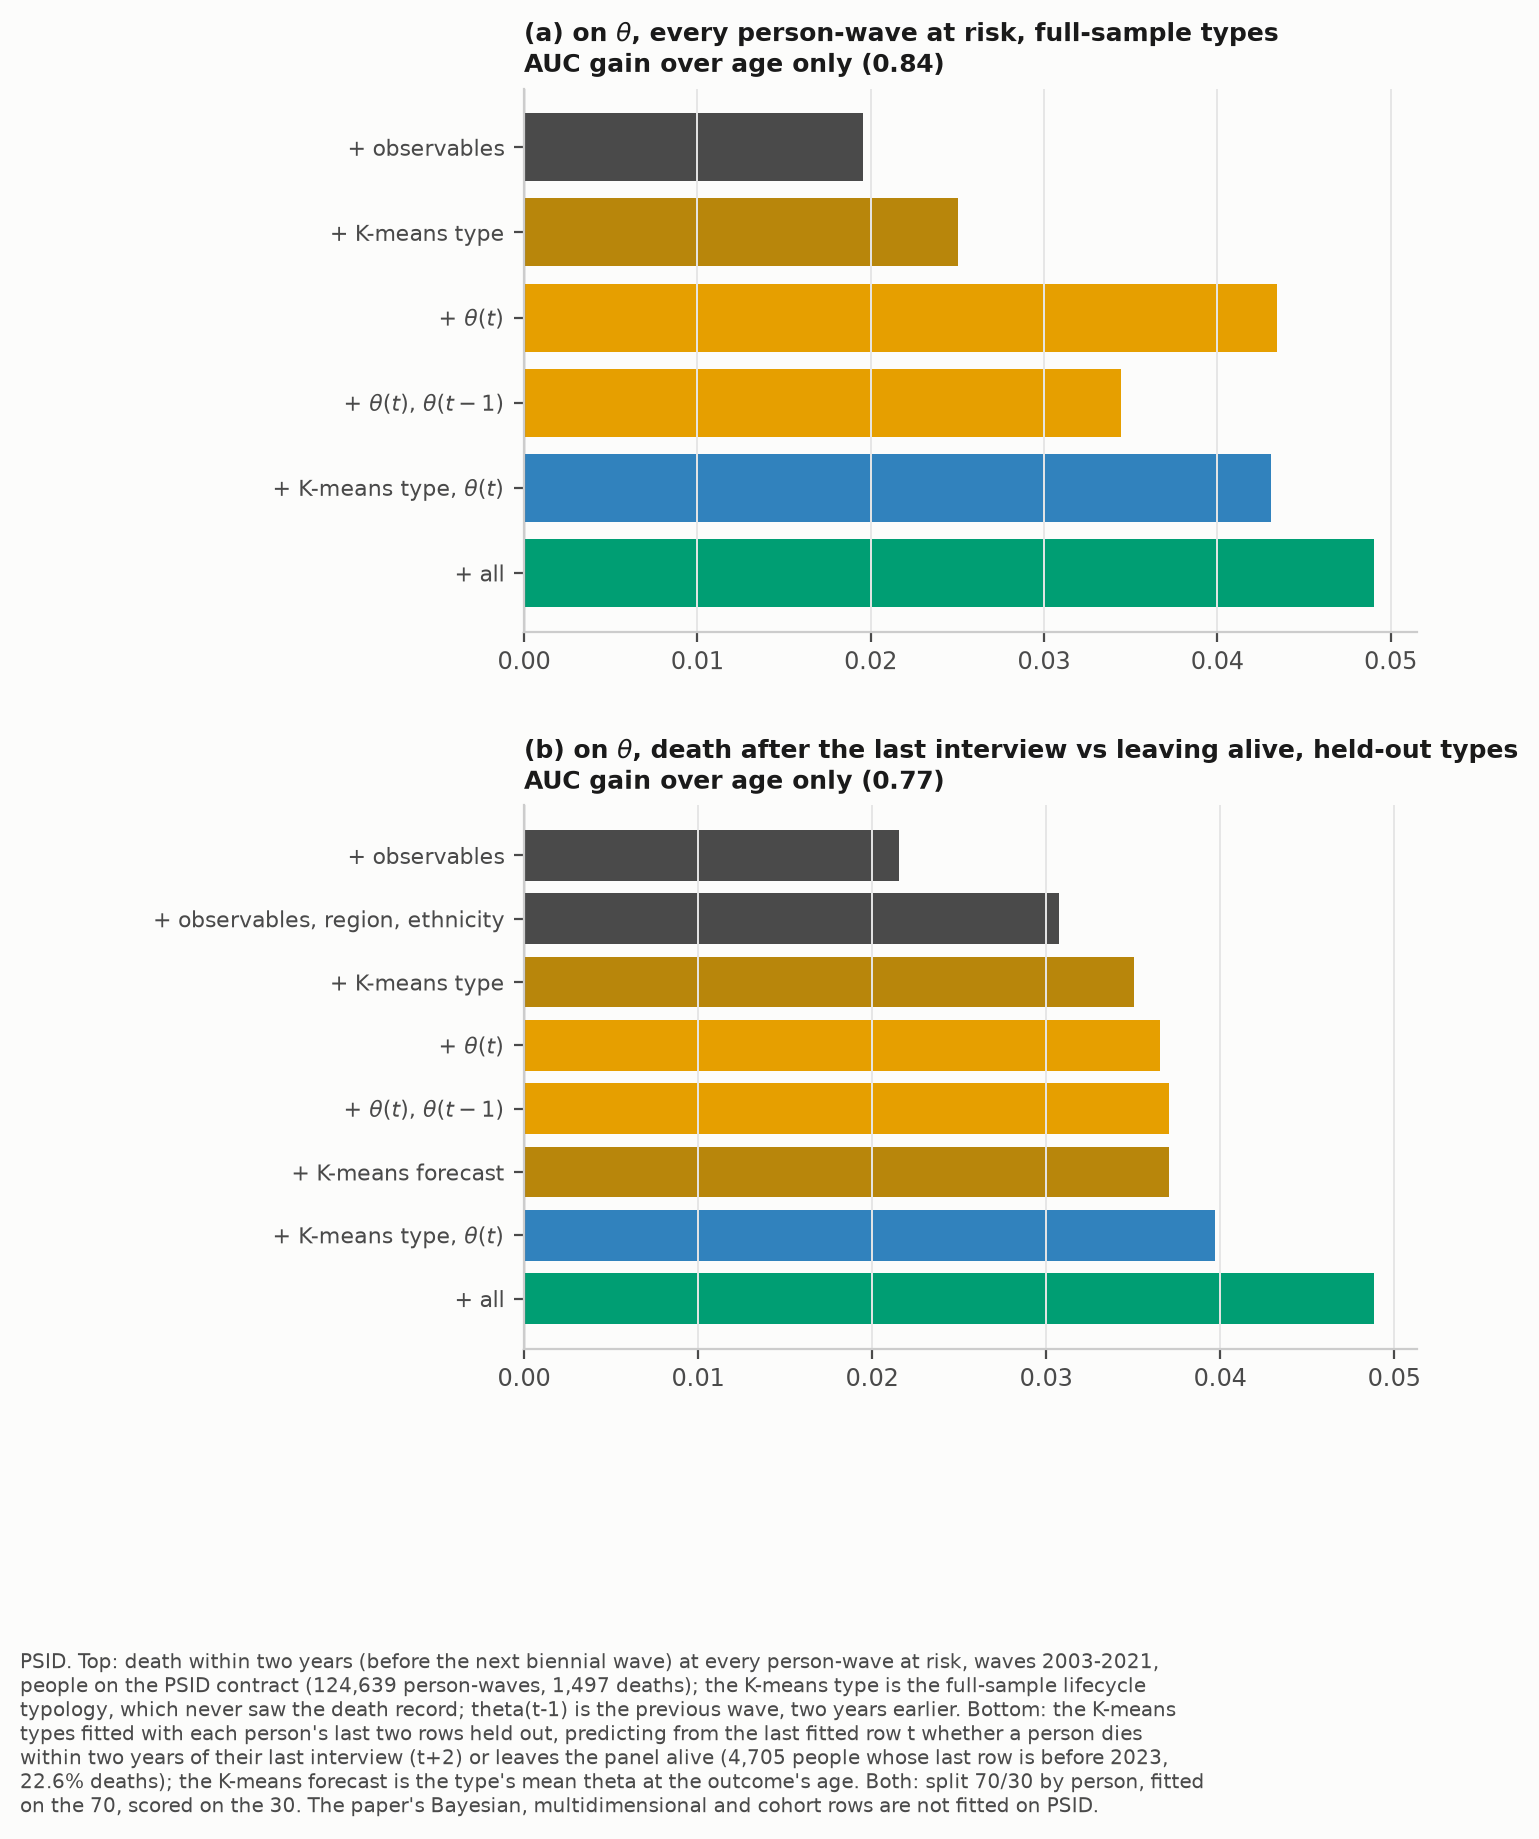
\includegraphics[height=0.62\textheight,keepaspectratio]{figures/main/fig_prediction_mortality.png}\end{center}
\textbf{Caption (PSID).} AUC gain over an age-only quadratic. (a) Every person-wave at risk with the full-sample K-means types: death within two years. (b) The K-means types fitted with each person's last two rows held out: death within two years of the last interview against leaving the panel alive, predicted from the last fitted row.

\textbf{What differs.} The Bayesian, multidimensional and cohort rows are dropped; K-means rows are added, since they are the only typology. Outcomes are two-year deaths. In (b) the held-out sample is people whose last row is before 2023: in PSID these are few (4,705) and a large share of them died (22.6 percent, against 7.2 percent in the UKHLS), because PSID loses few people to attrition and counts deaths over two years.

\textbf{What the comparison shows.} Base AUC 0.84 (UKHLS 0.85). $\theta_t$ adds 0.043 (UKHLS 0.044); the K-means type adds 0.025 (the UKHLS Bayesian classes add 0.025 to 0.030), and adds nothing once $\theta_t$ is in. Observables add more in PSID (0.020 against 0.004), consistent with a steeper US socioeconomic gradient in mortality. In (b) the gains are of the same size: $\theta_t$ adds 0.037 (UKHLS 0.030) and everything together 0.049 (UKHLS 0.033), on a much smaller sample.
\orig{fig_prediction_mortality.png}

%-----------------------------------------------------------------
\fig{12}{Trajectories of $\theta$ by type and by observable groups}
\begin{center}\psid{fig_observables.png}\end{center}
\textbf{Caption (PSID).} Lifecycle trajectories of $\theta$ by (a) K-means type, (b) the observable partitions (48 defined, 36 with cells large enough to draw), (c) education and (d) income decile, on the clustered people. Five-year centred rolling means of the age-specific cell means, cells with fewer than 30 people suppressed; (b) and (d) stop at 70.

\textbf{What differs.} Panel (a) has the K-means types only (the paper adds the AR(1) plus ``spike'' paths). Education is four US groups; partitions use white (non-Hispanic) against other; income is family income in the previous calendar year, before tax.

\textbf{What the comparison shows.} The paper's point holds: the observables spread $\theta$ far less than the types. The between-group share of the variance at 50 is 0.05 for education, 0.14 for income deciles and 0.15 for the 48 partitions together, against 0.61 for the three types (UKHLS 0.03, 0.08, 0.09 and 0.60), and the adjusted Rand index of every partition with the types is below 0.05. The gradients are about one and a half times steeper in PSID, especially by income.
\orig{fig_observables.png}

%-----------------------------------------------------------------
\fig{13}{Predicting ahead and predicting the type (adapted)}
\begin{center}\psid{fig_prediction_summary.png}\end{center}
\textbf{Caption (PSID).} (a) The gain in out-of-sample $R^2$ over a quadratic in age in predicting $\theta$ one (two years, full bars) and two (four years, light bars) waves ahead from what is known at a person's last fitted row; every fit held out each person's last two rows (13,529 people at $t+1$). (c) One wave ahead within age bands at $t$. (b) Balanced accuracy for the K-means type fitted with each person's first two rows held out (13,997 people), from the observables, the closest held reading $\theta_{t-1}$ and both readings. (d) Education, income third and sex within each K-means type of (b).

\textbf{What differs.} The AR(1) plus ``spike'' and multidimensional bars are dropped; (c) shows the K-means forecast in place of the AR(1) plus ``spike'' forecast; (d) shows the K-means types in place of the AR(1) plus ``spike'' types. A PSID wave is two years, so ``one wave ahead'' is a two-year forecast.

\textbf{What the comparison shows.} Gains at $t+1$: observables 0.10, $\theta_t$ 0.51, $\theta_t$ and $\theta_{t-1}$ 0.54, K-means forecast 0.41 (UKHLS 0.06, 0.55, 0.59, 0.45). A single reading again beats the type's centroid, and the observables add little, though more than in the UKHLS. Balanced accuracy for the type: 0.42 from observables, 0.64 from $\theta_{t-1}$, 0.66 from both readings (UKHLS K-means 0.39, 0.65, 0.68). In (d), 60 percent of the worst type is in the bottom income third and 18 percent has a degree, against 20 and 46 percent in the best type.
\orig{fig_prediction_summary.png}

%-----------------------------------------------------------------
\fig{14}{Prevention on the $K=3$ K-means types (adapted)}
\begin{center}\psid{fig_prevention.png}\end{center}
\textbf{Caption (PSID).} Prevention on the $K=3$ partial K-means types on $\theta$, in pounds under the PSID cubic cost curve of Figure 1 (in-patient only). (a) The saving at $\mu=0.1$ by type and start age $r$, uniform dashed. (b) The bill still to come $C(r)$, stacked into the cost at the mean path, what the type differences add and what realised deviations add, with the saving from uniform prevention at $\mu=1$. (c) The saving at $\mu=0.1$ in each year of age from prevention started at 25 and 60, by type. (d) Targeting at $\mu=0.1$ on the K-means types refitted with each person's first two rows held out, by what the prediction uses, with targeting on the estimated type dashed. Panel titles say ``class'' where they come from the paper's drawing functions; read ``type''.

\textbf{What differs.} K-means types in place of the AR(1) plus ``spike'' classes, so the ``realised deviations'' layer is around type means, not class paths, and the model-posterior targeting rules are dropped (they need a mixture). The cost curve is in-patient only. The UKHLS in-patient tier alone has no prevention run to compare with; the UKHLS numbers quoted are for its K-means appendix figure on the full index.

\textbf{What the comparison shows.} The structure carries over: the worst type's saving is far above the others' and falls fastest with the start age, most of the saving arrives late in life, and $\theta_{t-1}$ captures most of what targeting on the estimated type collects at small coverage. Levels, at $r=25$: bill \pounds53,500 (UKHLS full index, K-means \pounds67,500); saving at $\mu=0.1$ by type \pounds20,900, \pounds8,700, \pounds2,200, uniform \pounds8,800 (UKHLS K-means \pounds16,600, \pounds5,800, \pounds1,600, uniform about \pounds6,100); uniform saving at $\mu=1$ is 88 percent of the bill (UKHLS K-means 59 percent). The PSID bill is close to the UKHLS one despite pricing hospital stays only, because the PSID in-patient cost rises much more steeply in $\theta$ (Figure 1), and that steepness also makes the savings larger relative to the bill. The between-type layer is a larger part of the PSID bill (29 against 23 percent). Targeting the top 10 percent: \pounds9,400 per treated person on age alone, \pounds10,800 with observables, \pounds14,300 with $\theta_{t-1}$, \pounds18,400 on the estimated type; everyone treated \pounds6,200.
\orig{fig_prevention.png}

%-----------------------------------------------------------------
\clearpage\section*{Figure 15: prevention, life expectancy and inequality}
\textbf{Skipped.} The figure is built on the multidimensional Bayesian fit ($\theta$, the mental GRM and Gompertz--Makeham mortality), with hazards rescaled to the ONS national life tables for the UK. None of these exists for PSID and the brief excludes Bayesian and multidimensional fits.

\end{document}
